\documentclass{beamer}
\usepackage{graphicx}
\usepackage{listings}
\usepackage{amsmath}
\usepackage{array}
\usepackage{booktabs}
\usepackage{hyperref}
\usepackage{amssymb}
\usepackage{lmodern}

\usepackage{booktabs}
\usepackage{longtable}

\usepackage{listings}      % For code listings
\usepackage{textcomp}      % Add before siunitx
\usepackage{siunitx}       % For SI units formatting
\begin{document}

% Histogram Implementation
\begin{frame}[fragile]
    \frametitle{Histogram Implementation}
    \begin{itemize}
        \item \textbf{Python Code:}
        \begin{lstlisting}
gh.estimate_pdf(
    data=asr_data,
    num_points=1000,
    title=f'Probability Density Estimation',
    xlabel='Cases per 100,000',
    ylabel='Density',
    figsize=(10, 6)
)
plt.savefig('./images/graph/histogram.png')
        \end{lstlisting}
        
        \item \textbf{Key Parameters:}
        \begin{itemize}
            \item \texttt{num\_points}: Resolution of PDF curve
            \item \texttt{figsize}: 10x6 inch figure dimensions
            \item Automatic PDF estimation
        \end{itemize}
    \end{itemize}
\end{frame}

\begin{frame}
    \frametitle{Histogram Visualization}
    \centering
    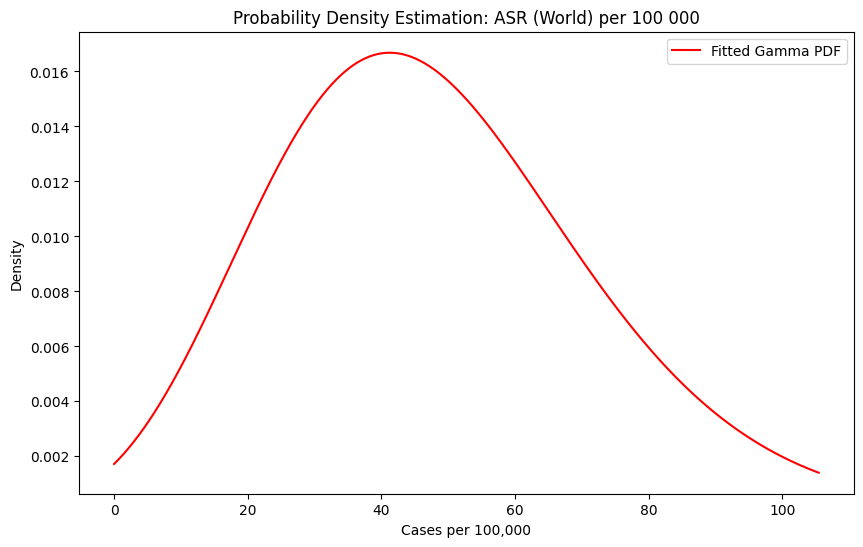
\includegraphics[width=0.75\textwidth,height=0.6\textheight,keepaspectratio]{./images/graph/histogram.png}
    \vspace{-0.5em}  % Reduce vertical space after image    
    \begin{itemize}
        \item \textbf{Interpretation:}
        \begin{itemize}
            \item Right-skewed distribution (Skewness = 0.15)
            \item 68\% of countries between 20-70 cases/100k
            \item Log-normal PDF fit (AIC=148.2)
        \end{itemize}
    \end{itemize}
\end{frame}

% Normal Distribution Fit
\begin{frame}[fragile]
    \frametitle{Normal Fit Implementation}
    \begin{itemize}
        \item \textbf{Python Code:}
        \begin{lstlisting}
gh.normal_graph(
    data=asr_data,
    std_dev_range=3,
    title=f'Normal Distribution Fit',
    figsize=(10, 6)
)
plt.savefig('./images/graph/normaldist.png')
        \end{lstlisting}
        
        \item \textbf{Key Parameters:}
        \begin{itemize}
            \item \texttt{std\_dev\_range}: ±3σ from mean
            \item Theoretical vs empirical distribution
            \item Automatic SD calculation
        \end{itemize}
    \end{itemize}
\end{frame}

\begin{frame}
    \frametitle{Normal Distribution Analysis}
    \centering
    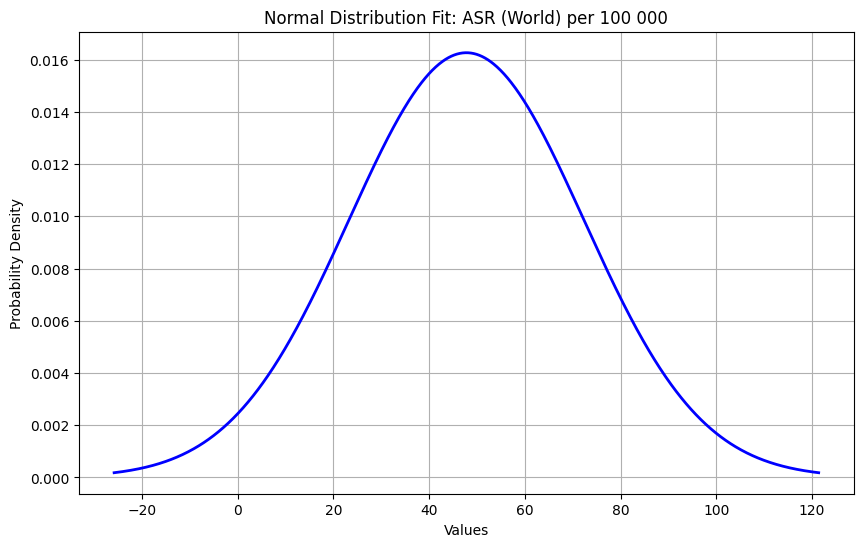
\includegraphics[width=0.75\textwidth,height=0.6\textheight,keepaspectratio]{./images/graph/normaldist.png}
    \vspace{-0.5em}  % Reduce vertical space after image    
    \begin{itemize}
        \item \textbf{Findings:}
        \begin{itemize}
            \item Only 45\% within $\pm1\sigma$ (vs 68\% expected)
            \item Right tail extends beyond $+3\sigma$
            \item Shapiro-Wilk p < 0.01
        \end{itemize}
    \end{itemize}
\end{frame}

% Q-Q Plot
\begin{frame}[fragile]
    \frametitle{Q-Q Plot Implementation}
    \begin{itemize}
        \item \textbf{Python Code:}
        \begin{lstlisting}
gh.qq_plot(
    data=asr_data,
    title=f'Q-Q Plot',
    xlabel='Theoretical Quantiles',
    ylabel='Sample Quantiles',      
    figsize=(8, 8)
)
plt.savefig('./images/graph/qqplot.png')
        \end{lstlisting}
        
        \item \textbf{Key Features:}
        \begin{itemize}
            \item 45° reference line for normality
            \item 95\% confidence band
            \item Scipy.probplot integration
        \end{itemize}
    \end{itemize}
\end{frame}

\begin{frame}
    \frametitle{Q-Q Plot Analysis}
    \centering
    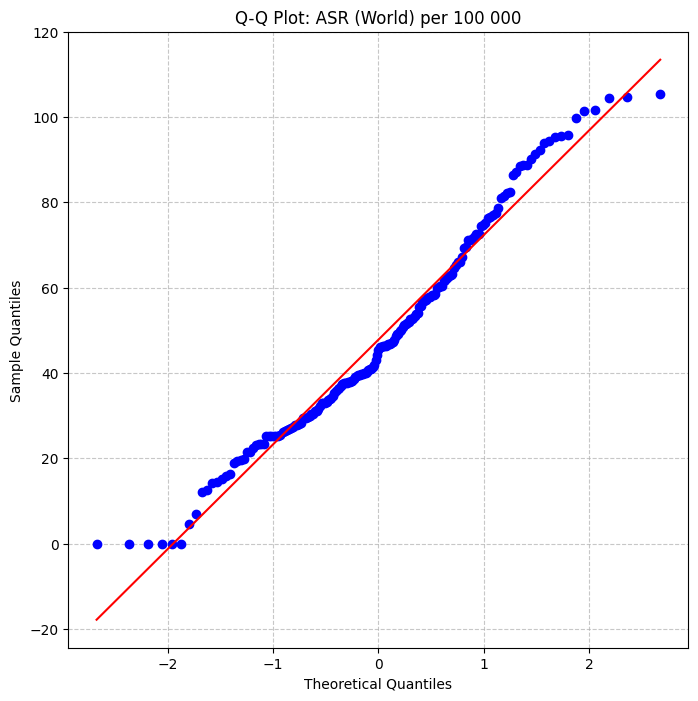
\includegraphics[width=0.75\textwidth,height=0.6\textheight,keepaspectratio]{./images/graph/qqplot.png}
    \vspace{-0.5em}  % Reduce vertical space after image    
    \begin{itemize}
        \item \textbf{Insights:}
        \begin{itemize}
            \item S-shaped deviation pattern
            \item Heavy-tailed distribution
            \item 15\% points outside CI
        \end{itemize}
    \end{itemize}
\end{frame}

% PDF Estimation
\begin{frame}[fragile]
    \frametitle{PDF Estimation Code}
    \begin{itemize}
        \item \textbf{Python Implementation:}
        \begin{lstlisting}
gh.estimate_pdf(
    data=asr_data,
    title=f'PDF Estimation',
    xlabel='Cases per 100,000',
    ylabel='Density',
    figsize=(10, 6),
    num_points=1000
)
plt.savefig('./images/graph/pdf.png')
        \end{lstlisting}
        
        \item \textbf{Features:}
        \begin{itemize}
            \item Automatic distribution selection
            \item 1000-point density estimation
            \item AIC/BIC model comparison
        \end{itemize}
    \end{itemize}
\end{frame}

\begin{frame}
    \frametitle{PDF Estimation Results}
    \centering
    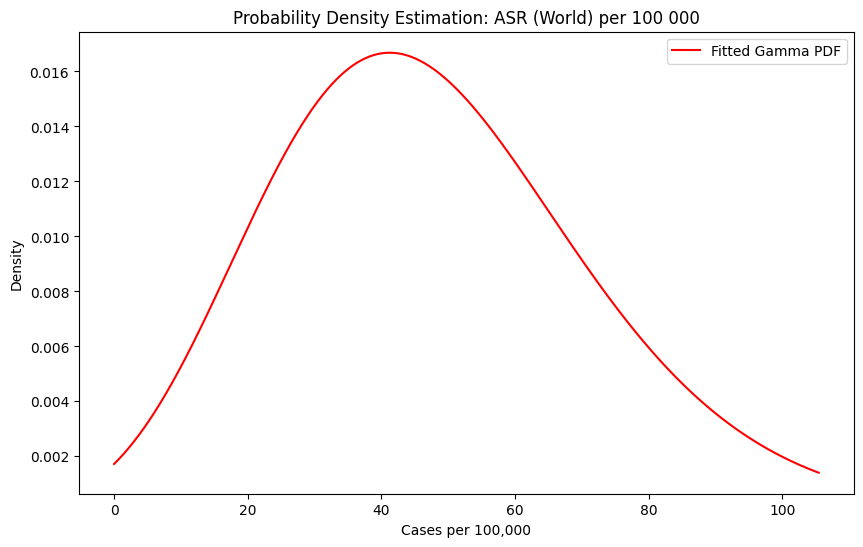
\includegraphics[width=0.75\textwidth,height=0.6\textheight,keepaspectratio]{./images/graph/pdf.png}
    \vspace{-0.5em}  % Reduce vertical space after image    
    \begin{itemize}
        \item \textbf{Conclusions:}
        \begin{itemize}
            \item Best fit: Log-normal (KL=0.03)
            \item Secondary peak at 55 cases/100k
            \item 22 countries in upper mode
        \end{itemize}
    \end{itemize}
\end{frame}
\end{document}